\documentclass[10pt,a4paper,twocolumn,twoside]{article}
\usepackage[utf8]{inputenc}
\usepackage[spanish]{babel}
\usepackage{multicol}
\usepackage{graphicx}
\usepackage{fancyhdr}
\usepackage{times}
\usepackage{titlesec}
\usepackage{multirow}
\usepackage{lettrine}
\usepackage[top=2cm, bottom=1.5cm, left=2cm, right=2cm]{geometry}
\usepackage[figurename=Fig.,tablename=TAULA]{caption}
\usepackage{url}
\usepackage{tabularx}
\usepackage{array}
\usepackage{caption}

\author{\LARGE\sffamily Luis Martínez Zamora}
\title{\Huge{\sffamily Data-Centric AI\@: Mejora de modelos de diagnostico médico mediante pipelines de curación e ingestión automática de vídeo}}
  

\newcommand\blfootnote[1]{%
  \begingroup
  \renewcommand\thefootnote{}\footnote{#1}%
  \addtocounter{footnote}{-1}%
  \endgroup
}

%
%\large\bfseries\sffamily
\titleformat{\section}
{\large\sffamily\scshape\bfseries}
{\textbf{\thesection}}{1em}{}

\begin{document}

\fancyhead[LO]{\scriptsize Luis Martínez Zamora: Data Centric AI\@: Mejora de modelos de diagnostico médico mediante pipelines de curación e ingestión automática de vídeo}
\fancyhead[RO]{\thepage}
\fancyhead[LE]{\thepage}
\fancyhead[RE]{\scriptsize EE/UAB TFG INFORMÀTICA\@: Data-Centric AI}

\fancyfoot[CO,CE]{}

\fancypagestyle{primerapagina}
{
  \fancyhf{}
  \fancyhead[L]{\scriptsize TFG EN ENGINYERIA INFORMÀTICA, ESCOLA D'ENGINYERIA (EE), UNIVERSITAT AUTÒNOMA DE BARCELONA (UAB)}
  \fancyfoot[C]{\scriptsize Marzo~de~2026, Escola d'Enginyeria (UAB)}
}

%\lhead{\thepage}
%\chead{}
%\rhead{\tiny EE/UAB TFG INFORMÀTICA: TÍTOL (ABREUJAT SI ÉS MOLT LLARG)}
%\lhead{ EE/UAB \thepage}
%\lfoot{}
%\cfoot{\tiny{Mes~2026, Escola d'Enginyeria (UAB)}}
%\rfoot{}
\renewcommand{\headrulewidth}{0pt}
\renewcommand{\footrulewidth}{0pt}
\pagestyle{fancy}

%\thispagestyle{myheadings}
\twocolumn[\begin{@twocolumnfalse}

%\vspace*{-1cm}{\scriptsize TFG EN ENGINYERIA INFORMÀTICA, ESCOLA D'ENGINYERIA (EE), UNIVERSITAT AUTÒNOMA DE BARCELONA (UAB)}

\maketitle

\thispagestyle{primerapagina}
%\twocolumn[\begin{@twocolumnfalse}
%\maketitle
%\begin{abstract}
\begin{center}
\parbox{0.915\textwidth}
{\sffamily
\textbf{Resumen--} Este proyecto propone un proceso automatizado basado en el paradigma Data-Centric AI para mejorar la clasificación multiclase de pólipos colorrectales. A través de las técnicas de Visión por Computador clásica se está transformando un conjunto de datos clínicos desequilibrados en homogéneos. El objetivo es demostrar empíricamente que la curación sistemática de los datos de entrenamiento maximiza el rendimiento de un modelo base.
\\
\\
\textbf{Palabras clave-- } Data-Centric AI, Computer Vision, Pytorch, Colonoscopia, Clasificación multiclase \\
\\
%\end{abstract}
%\bigskip
%\begin{abstract}
\bigskip
\\
\textbf{Abstract--} This project proposes an automated pipeline based on the Data-Centric AI paradigm to improve the multiclass classification of colorectal polyps. Using classical Computer Vision techniques, a highly imbalanced clinical dataset is transformed into a homogeneous one. The objective is to empirically demonstrate how systematic data curation maximizes the performance of a lightweight baseline model.
\\
\\
\textbf{Keywords-- } Data-Centric AI, Computer Vision, Pytorch, Colonoscopy, Multiclass Classification.\\
}


{\vrule depth 0pt height 0.5pt width 4cm\hspace{7.5pt}%
\raisebox{-3.5pt}{\fontfamily{pzd}\fontencoding{U}\fontseries{m}\fontshape{n}\fontsize{11}{12}\selectfont\char70}%
\hspace{7.5pt}\vrule depth 0pt height 0.5pt width 4cm\relax}

\end{center}

%\end{abstract}
\end{@twocolumnfalse}]

\section{Introducción y objetivos}

\blfootnote{$\bullet$ E-mail de contacte: lmzamoraa@gmail.com}
\blfootnote{$\bullet$ Menció: Computació}
\blfootnote{$\bullet$ Treball tutoritzat per: Yael Tudela (Ciències de la Computació)}
\blfootnote{$\bullet$ Curs 2025/26}

\lettrine[lines=3]{E}{l} cáncer colorrectal es el tercer cáncer más común a nivel mundial según la Organización Mundial de la Salud (OMS)\cite{who_colorectal_2024}, situándose además entre las principales causas de mortalidad oncológica. Por ello, la prevención y la detección temprana de esta enfermedad resultan fundamentales para reducir su impacto clínico.

En la práctica clínica, la colonoscopia no suele constituir siempre la primera prueba de detección del cáncer colorrectal. Existen distintas estrategias de cribado, entre ellas las pruebas basadas en heces, que son menos invasivas\cite{american_cancer_society_colon}. Sin embargo, cuando el resultado de estas pruebas sugiere la posible presencia de cáncer o de lesiones precursoras, es necesario realizar una colonoscopia para confirmar el hallazgo y continuar el estudio diagnóstico. Por este motivo, aunque no siempre representa la puerta de entrada al proceso asistencial, la colonoscopia ocupa un papel central en el diagnóstico del cáncer colorrectal, ya que permite identificar pólipos y otras lesiones directamente sobre la mucosa e incluso contribuir a la prevención de la enfermedad al detectar lesiones precancerosas.

La colonoscopia\cite{mayoclinic_colonoscopia} es un procedimiento médico cuyo objetivo es examinar el interior del intestino grueso y el recto. Para ello, se introduce por el ano un instrumento denominado colonoscopio, un tubo flexible equipado con una cámara y una fuente de luz en su extremo. Esta técnica permite la visualización directa y en tiempo real de la mucosa intestinal, lo que la convierte en una herramienta especialmente útil para detectar úlceras, inflamaciones, tumores y, en el contexto de este trabajo, pólipos. La identificación precisa de estas lesiones precancerosas durante la exploración en vídeo es crítica, ya que su detección temprana reduce de forma significativa el riesgo de progresión a cáncer colorrectal.

Actualmente, la evaluación de pólipos durante una colonoscopia se realiza principalmente mediante la observación visual del médico especialista. Sin embargo, esta tarea puede resultar compleja debido a la variabilidad en la apariencia anatómica de las lesiones, las condiciones de iluminación y la presencia de artefactos visuales. En este contexto, el uso de técnicas de inteligencia artificial para asistir en el análisis automatizado de colonoscopias ha despertado un interés creciente.

Respecto a las posibles lesiones, los pólipos no son un grupo homogéneo, sino que presentan diversas histologías que exigen protocolos de actuación y tratamientos distintos. Gran parte de los sistemas automatizados existentes se han limitado a desarrollar clasificadores binarios que discriminan únicamente entre lesiones neoplásicas (como los adenomas precancerosos) y no neoplásicas (pólipos benignos). No obstante, la realidad clínica es más compleja que una simple distinción binaria entre lesiones neoplásicas y no neoplásicas. En el contexto de este trabajo, se ha optado por una clasificación en cuatro clases —adenomas, adenomas serrados sésiles, pólipos hiperplásicos y adenocarcinomas— porque cada una de ellas representa una situación clínica diferente y aporta un nivel de detalle diagnóstico relevante. Los pólipos hiperplásicos suelen asociarse a un potencial maligno muy bajo, mientras que los adenomas constituyen precursores del cáncer colorrectal. Por su parte, las lesiones serradas sésiles también pueden actuar como precursoras, pero a través de una vía biológica distinta y con una apariencia más sutil, lo que incrementa su dificultad de detección. Finalmente, el adenocarcinoma representa una lesión maligna ya establecida, con implicaciones clínicas claramente diferenciadas respecto al resto de categorías consideradas en este trabajo, que corresponden a lesiones benignas o premalignas. Por ello, limitar el problema a dos clases reduciría la complejidad real del escenario clínico y ocultaría diferencias relevantes para el diagnóstico y la toma de decisiones médicas.\cite{rex2012,nih_colon_treatment}

Computacionalmente, esta transición de una clasificación binaria a una multiclase introduce un problema crítico: cada variante presenta diferencias sutiles y una frecuencia de aparición muy dispar en la población general. Esto genera un severo desbalanceo natural de las muestras, donde la escasez de imágenes para las tipologías menos comunes provoca que los clasificadores estándar pierdan eficacia.

Los conjuntos de datos clínicos presentan dificultades estructurales que los diferencian de otros problemas de visión artificial más controlados. En primer lugar, suelen estar marcados por un fuerte desbalanceo de clases, ya que las lesiones más frecuentes concentran gran parte de las muestras mientras que las patologías menos comunes aparecen escasamente representadas. Esto, sumado a la variabilidad de cada lesión entre pacientes y la necesidad de anotaciones expertas, limita la disponibilidad de datos. En consecuencia, el rendimiento de los modelos no depende únicamente de la arquitectura utilizada, sino también de la calidad y representatividad del conjunto de entrenamiento.\cite{salmi2024imbalanced}

Tradicionalmente, gran parte de la investigación en inteligencia artificial médica ha abordado este tipo de problemas desde un enfoque \textit{model-centric}. Bajo este paradigma, la mejora del sistema se persigue principalmente mediante modificaciones en la arquitectura, ajustes de hiperparámetros, estrategias de entrenamiento más complejas o combinaciones de múltiples modelos. Aunque este enfoque puede producir mejoras en entornos experimentales, en el ámbito clínico presenta limitaciones como el incremento del coste computacional, lo que dificulta el despliegue en tiempo real y, sobre todo, no corrige de forma directa los defectos estructurales del conjunto de datos. Cuando el origen del problema se encuentra en el ruido, la redundancia o el desbalanceo de las muestras, aumentar la complejidad del modelo no siempre se traduce en una mejora robusta del sistema.\cite{zha2025datacentric}

Frente a esta perspectiva, el paradigma \textit{Data-Centric AI} propone trasladar el foco principal de la ingeniería desde el modelo hacia los datos. Este enfoque se basa en diseñar y refinar sistemáticamente los datos, asumiendo una arquitectura relativamente estable y concentrando el esfuerzo en mejorar la calidad del conjunto de entrenamiento.\cite{ng_datacentric} Esta visión ha sido posteriormente consolidada por la comunidad investigadora, que la describe como una transición desde la mejora del modelo hacia el tratamiento de problemas como la recolección de datos, el etiquetado, el preprocesado y la evaluación de calidad del dato.\cite{zha2025datacentric}

Este trabajo se sitúa explícitamente dentro de este último paradigma. En lugar de plantear sucesivas iteraciones sobre arquitecturas cada vez más complejas, se fija un modelo \textit{baseline} ligero y se concentra la contribución principal en la construcción de un pipeline de software orientado a mejorar los datos de entrenamiento. Dicho pipeline aborda de forma secuencial la ingestión automática de imágenes a partir de vídeo, la reducción de redundancia temporal, el filtrado de calidad de imagen y el reequilibrado de clases. De este modo, la hipótesis central del TFG no es que un modelo más complejo resuelva mejor el problema, sino que una mejora sistemática y reproducible de los datos clínicos puede aumentar de forma significativa la capacidad predictiva de un clasificador estándar.\cite{zha2025datacentric, ng_datacentric}

\subsection{Objetivos}
\subsubsection{Objetivo principal}
Desarrollar un pipeline automatizado de curación e ingestión de datos a partir de vídeo bajo el paradigma Data-Centric AI, evaluando de forma iterativa la evolución del rendimiento de un modelo baseline específico, en este caso será una arquitectura ligera pre-entrenada del tipo EfficientNet\cite{tan2019efficientnet}, fijando los hiperparámetros que se utilizarán a lo largo de todo el proceso. La elección de esta arquitectura ligera busca reducir la carga computacional, permitiendo iteraciones rápidas para evaluar el impacto de las mejoras en los datos.

El propósito es cuantificar la mejora progresiva del clasificador paso a paso mediante métricas de evaluación robustas frente al desbalanceo de clases, específicamente F1-score macro, además de la matriz de confusión para analizar el comportamiento por clase. Con esto se busca demostrar empíricamente que la optimización sistemática de los datos de entrenamiento es un factor determinante para maximizar la capacidad predictiva del sistema, superando al conjunto de datos original estático.
\subsubsection{Objetivos secundarios}
\begin{itemize}
    \item Construir un módulo de software eficiente para la ingestión y procesamiento de vídeos de colonoscopias que permita la extracción inteligente de frames a partir de las marcas temporales (timestamps) etiquetadas por los especialistas. En lugar de una extracción contigua basada en ventanas fijas, el sistema implementará técnicas de Visual Object Tracking (VOT) basadas en el paradigma Tracking-by-Detection, con un modelo de detección YOLO junto al algoritmo ByteTrack\cite{zhang2022bytetrack}, ya que este seguirá el rastro del pólipo en situaciones donde la calidad de la imagen baja drásticamente, permitiendo encontrar imagenes de buena calidad. Esto permitirá buscar en la cercanía temporal del frame original para extraer perspectivas alternativas del mismo pólipo y, simultáneamente, corregir errores de etiquetado manual seleccionando automáticamente el frame de mayor calidad óptica si el original carece de valor diagnóstico. Hay que destacar que esta etapa de extracción será más restrictiva con clases mayoritarias, buscando reducir así el desbalanceo.
    \item Implementar algoritmos de similitud visual, haciendo uso de técnicas como Perceptual Hashing (pHash) o métricas como Structural Similarity Index Measure (SSIM), para identificar secuencias de frames temporalmente redundantes. Sobre estos grupos, se aplicará una política de selección para extraer los $X$ frames de mayor calidad óptica. Esta selección se automatizará calculando un Quality Score basado en la maximización de la nitidez (mediante la Varianza del Laplaciano) y el área de la lesión detectada, garantizando así la máxima riqueza visual para el entrenamiento y previniendo el overfitting.
    \item Implementar un algoritmo secuencial de descarte mediante técnicas de Visión Artificial clásica para la limpieza de los datos. El pipeline funcionará eliminando automáticamente frames sin valor diagnóstico en un orden específico: descarte por oscuridad, falta de textura por colisión contra la mucosa y desenfoque por movimiento de la cámara.
    \item Definir y ejecutar un marco de experimentación que registre y compare las métricas del modelo tras la aplicación sucesiva de cada módulo del pipeline, aislando y demostrando el impacto individual de cada técnica.
\end{itemize}

\section{Planificación temporal}
Para asegurar el correcto desarrollo del TFG, se ha establecido un cronograma (Fig.\ref{fig:gantt_tfg}) que divide el trabajo en bloques.

\begin{figure}[htbp]
    \centering
    \includegraphics[width=0.49\textwidth]{timeline.pdf}
    \caption{Diagrama de Gantt del desarrollo del TFG.}
    \label{fig:gantt_tfg}
\end{figure}

\subsection{Seguimiento de la planificación}
Hasta la fecha de entrega de este informe, el desarrollo del TFG ha seguido de forma general la planificación definida en el informe inicial, aunque se ha reajustado el orden de dos fases intermedias. En la versión actual del pipeline, la reducción de redundancia temporal se aplica antes del filtrado de calidad de imagen. Este cambio permite seleccionar primero los frames más representativos dentro de grupos visualmente similares y aplicar después los filtros de calidad sobre un conjunto menos redundante.

\begin{table}[htbp]
\centering
\caption{Seguimiento de la planificación en la tercera entrega}
\label{tab:seguimiento_planificacion}
\scriptsize
\resizebox{\columnwidth}{!}{%
\begin{tabular}{l l}
\hline
\textbf{Fase} &  \textbf{Estado actual}  \\
\hline
Fase 1: Baseline  & Completada  \\
Fase 2: Ingestión  & Completada  \\
Fase 3: Deduplicación  & Completada \\
Fase 4: Filtrado de calidad  & En desarrollo  \\
Fase 5: MLOps y análisis  & Pendiente \\
\hline
\end{tabular}%
}
\end{table}

Por tanto, no se modifica la estructura global del plan de trabajo, pero sí la secuencia interna del pipeline para adaptarla al comportamiento observado durante el desarrollo experimental.
\section{Metodología seguida}
\subsection{Fase 1: Entrenamiento del modelo baseline}

\subsubsection{Arquitectura seleccionada}
Como punto de partida del proyecto se define un modelo \textit{baseline} fijo, que actúa como referencia sobre la que se evaluará el impacto de todas las mejoras introducidas posteriormente en los datos. Dado que el objetivo del TFG se enmarca en el paradigma \textit{Data-Centric AI}, no se persigue maximizar el rendimiento mediante iteraciones sucesivas sobre la arquitectura, sino mantener una receta de entrenamiento estable y reproducible para que la evolución de los resultados pueda atribuirse exclusivamente a los cambios aplicados al conjunto de datos.

Para ello se emplea una arquitectura \textit{EfficientNet-B0} preentrenada sobre ImageNet\cite{tan2019efficientnet}, elegida por su buena relación entre capacidad de aprendizaje y coste computacional. Esta elección resulta adecuada para el contexto del proyecto porque permite realizar múltiples iteraciones experimentales con un coste temporal asumible y, al mismo tiempo, suficiente para evaluar el efecto de la curación del dataset sin recurrir a modelos excesivamente complejos.

\subsubsection{Configuración del entrenamiento}
La configuración final del entrenamiento se resume en la Tabla~\ref{tab:baseline_config}, donde se recogen los hiperparámetros relevantes que definen la receta final del \textit{baseline}.

La selección del mejor modelo se realiza atendiendo al valor de F1-score macro en validación, al tratarse de un problema multiclase con fuerte desbalanceo entre clases. De forma complementaria, se analiza la matriz de confusión para estudiar el comportamiento del clasificador en cada categoría histológica.

\subsubsection{Protocolo de validación}
El conjunto de validación se define una única vez a partir del dataset inicial y se mantiene fijo durante todas las fases posteriores del proyecto. La partición se realiza mediante un esquema estratificado y agrupado por identidad clínica de la lesión, utilizando como grupo la combinación de paciente, día de exploración, región y fragmento de vídeo. Esta decisión evita que imágenes muy similares de una misma lesión aparezcan simultáneamente en entrenamiento y validación, reduciendo así el riesgo de fuga de información.

Las fases posteriores modifican únicamente el conjunto de entrenamiento. De este modo, la comparación entre fases se realiza siempre contra la misma referencia de validación y las variaciones observadas en las métricas pueden atribuirse a los cambios introducidos sobre los datos de entrenamiento.

\subsubsection{Estrategia de fine-tuning}
La optimización sigue un esquema de \textit{fine-tuning} progresivo. Durante las primeras épocas se entrena únicamente la cabeza de clasificación adaptada al problema multiclase, manteniendo congelado el resto de la red. Esta decisión permite estabilizar primero la capa final, que parte de cero y debe aprender correctamente sobre las características visuales hacia las cuatro clases histológicas consideradas.

Una vez finalizado este periodo inicial, se habilita el entrenamiento de la red completa. Esta transición permite aprovechar el conocimiento visual ya presente en los pesos preentrenados, ajustándolo progresivamente al dominio del proyecto, sin modificar desde el inicio todas el conocimiento interno del modelo. En la práctica, esta estrategia resulta más estable que entrenar toda la red desde la primera iteración, ya que reduce el riesgo de deteriorar las características generales base del modelo.

Para acompañar este cambio de fase se definen tasas de aprendizaje diferenciadas. Durante el \textit{warmup}, la cabeza de clasificación se entrena con una tasa de aprendizaje superior, mientras que en la fase de \textit{fine-tuning} completo tanto la cabeza como el \textit{backbone} pasan a optimizarse con valores más bajos, especialmente en el backbone, provocando así una optimización más suave. Esta jerarquía responde a la distinta naturaleza de ambas partes: la cabeza requiere cambios más intensos al estar especializada directamente en la tarea final, mientras que el \textit{backbone} solo necesita ajustes finos.

\subsubsection{Tratamiento del desbalanceo de clases}
Dado que el problema presenta un fuerte desbalanceo entre clases, se opta por combinar una función de pérdida ponderada (\textit{weighted loss}) con un muestreo ponderado mediante \textit{WeightedRandomSampler}. Esta decisión permite incrementar la exposición del modelo a las clases minoritarias durante el entrenamiento y, a la vez, penalizar más los errores cometidos sobre dichas clases.

El exponente de ponderación se fija en 1.0, siguiendo la configuración oficial utilizada en el código actual del proyecto. Por tanto, tanto los pesos de la función de pérdida como los pesos de muestreo se calculan de forma proporcional a la frecuencia inversa de cada clase.

La Tabla~\ref{tab:baseline_config} resume la configuración final del modelo \textit{baseline}. Esta receta se mantiene fija en todos los experimentos posteriores del proyecto, de manera que cualquier variación observada en las métricas de validación pueda interpretarse como consecuencia directa de las modificaciones introducidas sobre los datos y no de cambios en el proceso de entrenamiento.

\begin{table}[t]
\centering
\small
\setlength{\tabcolsep}{4pt}
\caption{Configuración final del modelo baseline}
\label{tab:baseline_config}
\begin{tabularx}{\columnwidth}{|>{\raggedright\arraybackslash}X|>{\centering\arraybackslash}p{3.2cm}|}
\hline
\textbf{Parámetro} & \textbf{Valor} \\
\hline
Arquitectura & EfficientNet-B0 \\
Epochs máximas & 100 \\
Batch size & 32 \\
Warmup epochs & 3 \\
Learning rate cabeza (warmup) & $1 \times 10^{-3}$ \\
Learning rate cabeza (fine-tuning) & $1 \times 10^{-4}$ \\
Learning rate backbone & $1 \times 10^{-5}$ \\
Weight decay & $5 \times 10^{-4}$ \\
Dropout & 0.3 \\
Stochastic depth & 0.1 \\
Label smoothing & 0.02 \\
Scheduler & ReduceLROnPlateau \\
Scheduler patience & 4 \\
Early stopping patience & 12 \\
Weighted sampler & Sí \\
Exponente de pesos de clase & 1.0 \\
Métrica principal & Macro F1 \\
\hline
\end{tabularx}
\end{table}


\subsection{Fase 2: Ingestión de imágenes a partir de vídeo}
\subsubsection{Objetivo de la fase}
La segunda fase del pipeline tiene como objetivo ampliar el conjunto de datos a partir de los vídeos clínicos disponibles. Mientras que el dataset original parte de imágenes ya etiquetadas por los especialistas, esta fase permite aprovechar la información contenida en las exploraciones del cólon completas para generar nuevas muestras útiles para el entrenamiento. La finalidad es obtener imágenes cercanas al instante clínicamente relevante y con alta probabilidad de contener el pólipo de interés.

\subsubsection{Recorte de la región clínica útil}
Antes de aplicar el detector, se realiza un preprocesado orientado a eliminar zonas irrelevantes del vídeo. En las imagenes aparecen bordes negros o márgenes del sistema de captura que no aportan información útil. Para reducir este ruido, el pipeline detecta automáticamente la región clínica útil a partir de la zona no negra dominante de la imagen y recorta los frames a dicha región de interés. De este modo, el proceso de detección mediante YOLO se concentra en la parte realmente informativa de la escena endoscópica y facilita la obtención de un buen resultado.

\subsubsection{Detección y seguimiento del pólipo}
Para la detección inicial de pólipos se utilizó un checkpoint ya entrenado de YOLOv8 obtenido de un trabajo previo. La elección de este modelo resulta coherente con el tipo de anotación disponible en Kvasir-SEG, ya que dicho dataset proporciona imágenes de pólipos con máscaras de segmentación y las correspondientes \textit{bounding boxes} derivadas de ellas. Esta información es suficiente para entrenar un detector que aprenda a localizar automáticamente la lesión en la imagen. En el trabajo de referencia, el detector se emplea como primera etapa del sistema: primero predice la caja que contiene el pólipo y, a partir de esa localización, se guía el módulo posterior encargado de segmentarlo con mayor precisión.\cite{kvasirseg2019,sajjad_yolo_sam2}

En la configuración actual del pipeline, el procesamiento se realiza sobre una ventana temporal de $\pm 3$ segundos alrededor del \textit{timestamp} anotado. Los frames de esa ventana se muestrean a 5 FPS y se procesan con un umbral de confianza de detección de 0.15. Esta configuración permite explorar el entorno temporal inmediato de la anotación sin procesar el vídeo completo, manteniendo un coste computacional acotado.

\subsubsection{Selección de la trayectoria principal}
A partir de las detecciones iniciales con el modelo mencionado, se emplea ByteTrack\cite{zhang2022bytetrack} para construir trayectorias temporales del objeto detectado. Este algoritmo permite recuperar objetos incluso cuando algunas detecciones presentan baja confianza, reduciendo así la fragmentación del seguimiento. Sin embargo, dentro de una misma ventana temporal pueden coexistir varias trayectorias candidatas, por la presencia simultánea de más de una lesión o por detecciones erróneas del modelo. Por este motivo, sobre la salida del \textit{tracker} se aplica una heurística cuyo objetivo es seleccionar la trayectoria más probable del pólipo asociado al \textit{timestamp} clínico. Para ello, se priorizan las trayectorias más persistentes, más próximas temporalmente a la anotación original y, en caso de empate, con mayor confianza media de detección.

Para evitar trayectorias demasiado débiles, solo se consideran candidatas aquellas que acumulan al menos dos detecciones en la ventana temporal analizada. Si no se obtiene una trayectoria válida, el pipeline aplica una estrategia de respaldo basada en seleccionar los frames muestreados más cercanos al \textit{timestamp}. De esta forma, la fase de ingestión sigue generando candidatos incluso cuando el seguimiento temporal no resulta suficientemente estable.

En resumen, la trayectoria principal se selecciona priorizando, por este orden, persistencia temporal, proximidad al \textit{timestamp} anotado y confianza media de detección.

\subsubsection{Selección final de frames}
A partir de la trayectoria principal seleccionada, se escogen los frames concretos que pasarán a formar parte del dataset ampliado. Esta selección persigue dos objetivos: mantener cercanía temporal respecto a la anotación original y evitar redundancia excesiva entre imágenes consecutivas. Para ello, los frames se ordenan según su proximidad al instante de referencia.

Cuando la selección procede de una trayectoria válida, se impone una separación mínima entre frames equivalente al intervalo de muestreo utilizado. Con ello se evita seleccionar imágenes consecutivas prácticamente idénticas dentro de la misma trayectoria antes de que actúe la fase posterior de deduplicación.

\subsubsection{Control de la ampliación por histología}

El número máximo de imágenes generadas a partir de cada anotación no es uniforme para todas las clases histológicas. Se establece una política diferenciada según la histología asociada, permitiendo generar más candidatos en aquellas clases con menor representación relativa dentro del conjunto de datos. Esta decisión está alineada con el enfoque data-centric del proyecto, ya que la ingestión desde vídeo no se plantea únicamente como una técnica de aumento general del volumen de datos, sino también como una herramienta para actuar sobre el desbalanceo de clases desde una fase temprana del pipeline.

En la implementación actual, el número de candidatos por histología se calcula de forma automática mediante una ponderación inversamente proporcional a la frecuencia de cada clase en el conjunto de entrenamiento. La clase mayoritaria se toma como referencia y las clases menos frecuentes reciben un número máximo de candidatos superior, con un límite superior para evitar generar demasiadas muestras redundantes a partir de una misma anotación.

\subsubsection{Generación del conjunto de datos ampliado}
Finalmente, los frames seleccionados se guardan como nuevas imágenes independientes y se incorporan a la metadata del proyecto, preservando la etiqueta histológica original y el resto de la información clínica necesaria para su uso posterior en entrenamiento y evaluación. Cada fila generada incluye el tipo de origen de la imagen, el vídeo asociado, el instante temporal, la confianza de detección y el área relativa de la \textit{bounding box}. Como resultado, esta fase produce un dataset ampliado de forma automática, trazable y controlada, en el que cada nueva imagen deriva de una anotación clínica existente y ha sido seleccionada siguiendo criterios temporales, espaciales y de consistencia visual.

\subsection{Fase 3: Reducción de redundancia temporal}
La tercera fase del pipeline tiene como objetivo reducir la redundancia generada durante la ingestión de vídeo. Al extraer varios frames próximos a una misma anotación clínica, es habitual que muchas imágenes representen prácticamente la misma escena endoscópica. Mantener todas estas muestras puede incrementar artificialmente el tamaño del dataset sin aportar variabilidad visual real y puede favorecer que el modelo se ajuste en exceso a secuencias casi idénticas.

\subsubsection{Agrupación temporal de frames comparables}
La deduplicación se aplica únicamente entre imágenes que pueden considerarse comparables desde el punto de vista clínico. Para ello, los frames se agrupan por paciente, día, región, fragmento de exploración, vídeo e histología. Dentro de cada grupo base se generan eventos temporales usando una tolerancia de 2 segundos respecto al tiempo transcurrido en el vídeo. De este modo, solo se comparan frames cercanos en el tiempo y asociados a la misma lesión o contexto clínico.

\subsubsection{Cálculo de similitud visual}
Dentro de cada grupo temporal se comparan todos los pares de imágenes. Para homogeneizar el cálculo, cada frame se convierte a escala de grises y se redimensiona a una resolución fija antes de calcular las métricas de similitud. Se utilizan dos criterios complementarios: SSIM, que mide la similitud estructural entre imágenes, y pHash, que resume perceptualmente la imagen mediante un hash robusto frente a pequeñas variaciones.

En la versión actual del pipeline, un par se considera redundante únicamente si cumple simultáneamente ambos criterios: SSIM mayor o igual que 0.75 y distancia de Hamming entre pHashes menor o igual que 8. Esta decisión hace que la deduplicación sea más conservadora, ya que exige acuerdo entre una medida estructural y una medida perceptual antes de eliminar información del conjunto de entrenamiento.

\subsubsection{Selección de imágenes representativas}
Los pares redundantes se agrupan como componentes conectadas de un grafo, donde cada imagen es un nodo y cada relación redundante es una arista. De esta forma, si un frame es similar a otro y este a un tercero, los tres se consideran parte del mismo grupo de redundancia, aunque no todos los pares del grupo tengan que cumplir directamente los umbrales entre sí. Dentro de cada grupo se calcula un \textit{quality score} que combina nitidez, área relativa de la detección y confianza del detector.

\[
Q_i = 0.50 \cdot \hat{L}_i + 0.30 \cdot \hat{A}_i + 0.20 \cdot \hat{C}_i
\]

Donde $\hat{L}_i$ representa la varianza del Laplaciano normalizada, $\hat{A}_i$ el área relativa normalizada de la \textit{bounding box} y $\hat{C}_i$ la confianza normalizada de detección. La normalización se realiza dentro de cada grupo de redundancia, ya que la comparación solo tiene sentido entre imágenes candidatas a representar el mismo evento visual.

La selección final no conserva siempre el mismo número de imágenes por grupo. El valor de \textit{top-K} se calcula por histología a partir del desbalanceo observado, de modo que las clases minoritarias puedan retener más variantes visuales que la clase mayoritaria. Así, la fase de deduplicación reduce redundancia sin eliminar de forma agresiva las clases menos representadas.

\subsection{Fase 4: Filtrado de calidad de imagen}
La cuarta fase aplica un filtrado de calidad sobre el conjunto ya deduplicado. A diferencia de la fase anterior, que elimina imágenes por redundancia visual, esta etapa descarta frames que no aportan información diagnóstica suficiente por problemas de iluminación, textura o nitidez. El objetivo es reducir el ruido visual que puede introducir patrones espurios durante el entrenamiento, manteniendo una política conservadora para no eliminar imágenes útiles por pequeñas imperfecciones propias del vídeo endoscópico.

\subsubsection{Cálculo de métricas de calidad}
Antes de aplicar los filtros, el pipeline calcula y almacena para cada imagen las métricas visuales necesarias. Estas métricas se guardan en la metadata del dataset, de modo que la decisión de filtrado queda trazable y puede revisarse posteriormente.

La primera métrica es la media del canal V en el espacio HSV, utilizada como estimador de brillo global. La segunda es la entropía de Shannon sobre la imagen en escala de grises, que mide la cantidad de información estructural presente en la escena. La tercera es la varianza del Laplaciano, empleada como aproximación de nitidez: valores bajos indican menor presencia de bordes y, por tanto, mayor probabilidad de desenfoque.

\subsubsection{Aplicación secuencial de filtros}
El filtrado se aplica de forma secuencial. Si una imagen no supera uno de los criterios, queda descartada y no pasa a los filtros posteriores. Este diseño evita aplicar cálculos o decisiones posteriores sobre imágenes que ya han sido consideradas no aptas, y permite interpretar cuántas imágenes elimina cada criterio dentro del orden definido.

En la configuración actual se utilizan tres filtros. En todos los casos, los umbrales se seleccionan a partir de la distribución empírica de la métrica y de la inspección visual de ejemplos cercanos al punto de corte. Esta comparación permite equilibrar dos riesgos opuestos: conservar imágenes sin valor diagnóstico o eliminar frames que todavía contienen información útil.

\textbf{Filtro de oscuridad.} Detecta imágenes con iluminación insuficiente. La imagen se transforma al espacio HSV y se calcula la media del canal V. Si este valor es inferior a $T_{oscuro}=55$, el frame se descarta. Para fijar el umbral se comparan los valores candidatos 50, 55 y 60, como se muestra en la Figura~\ref{fig:phase4_darkness_threshold}.

\begin{center}
\begin{minipage}{\linewidth}
\centering
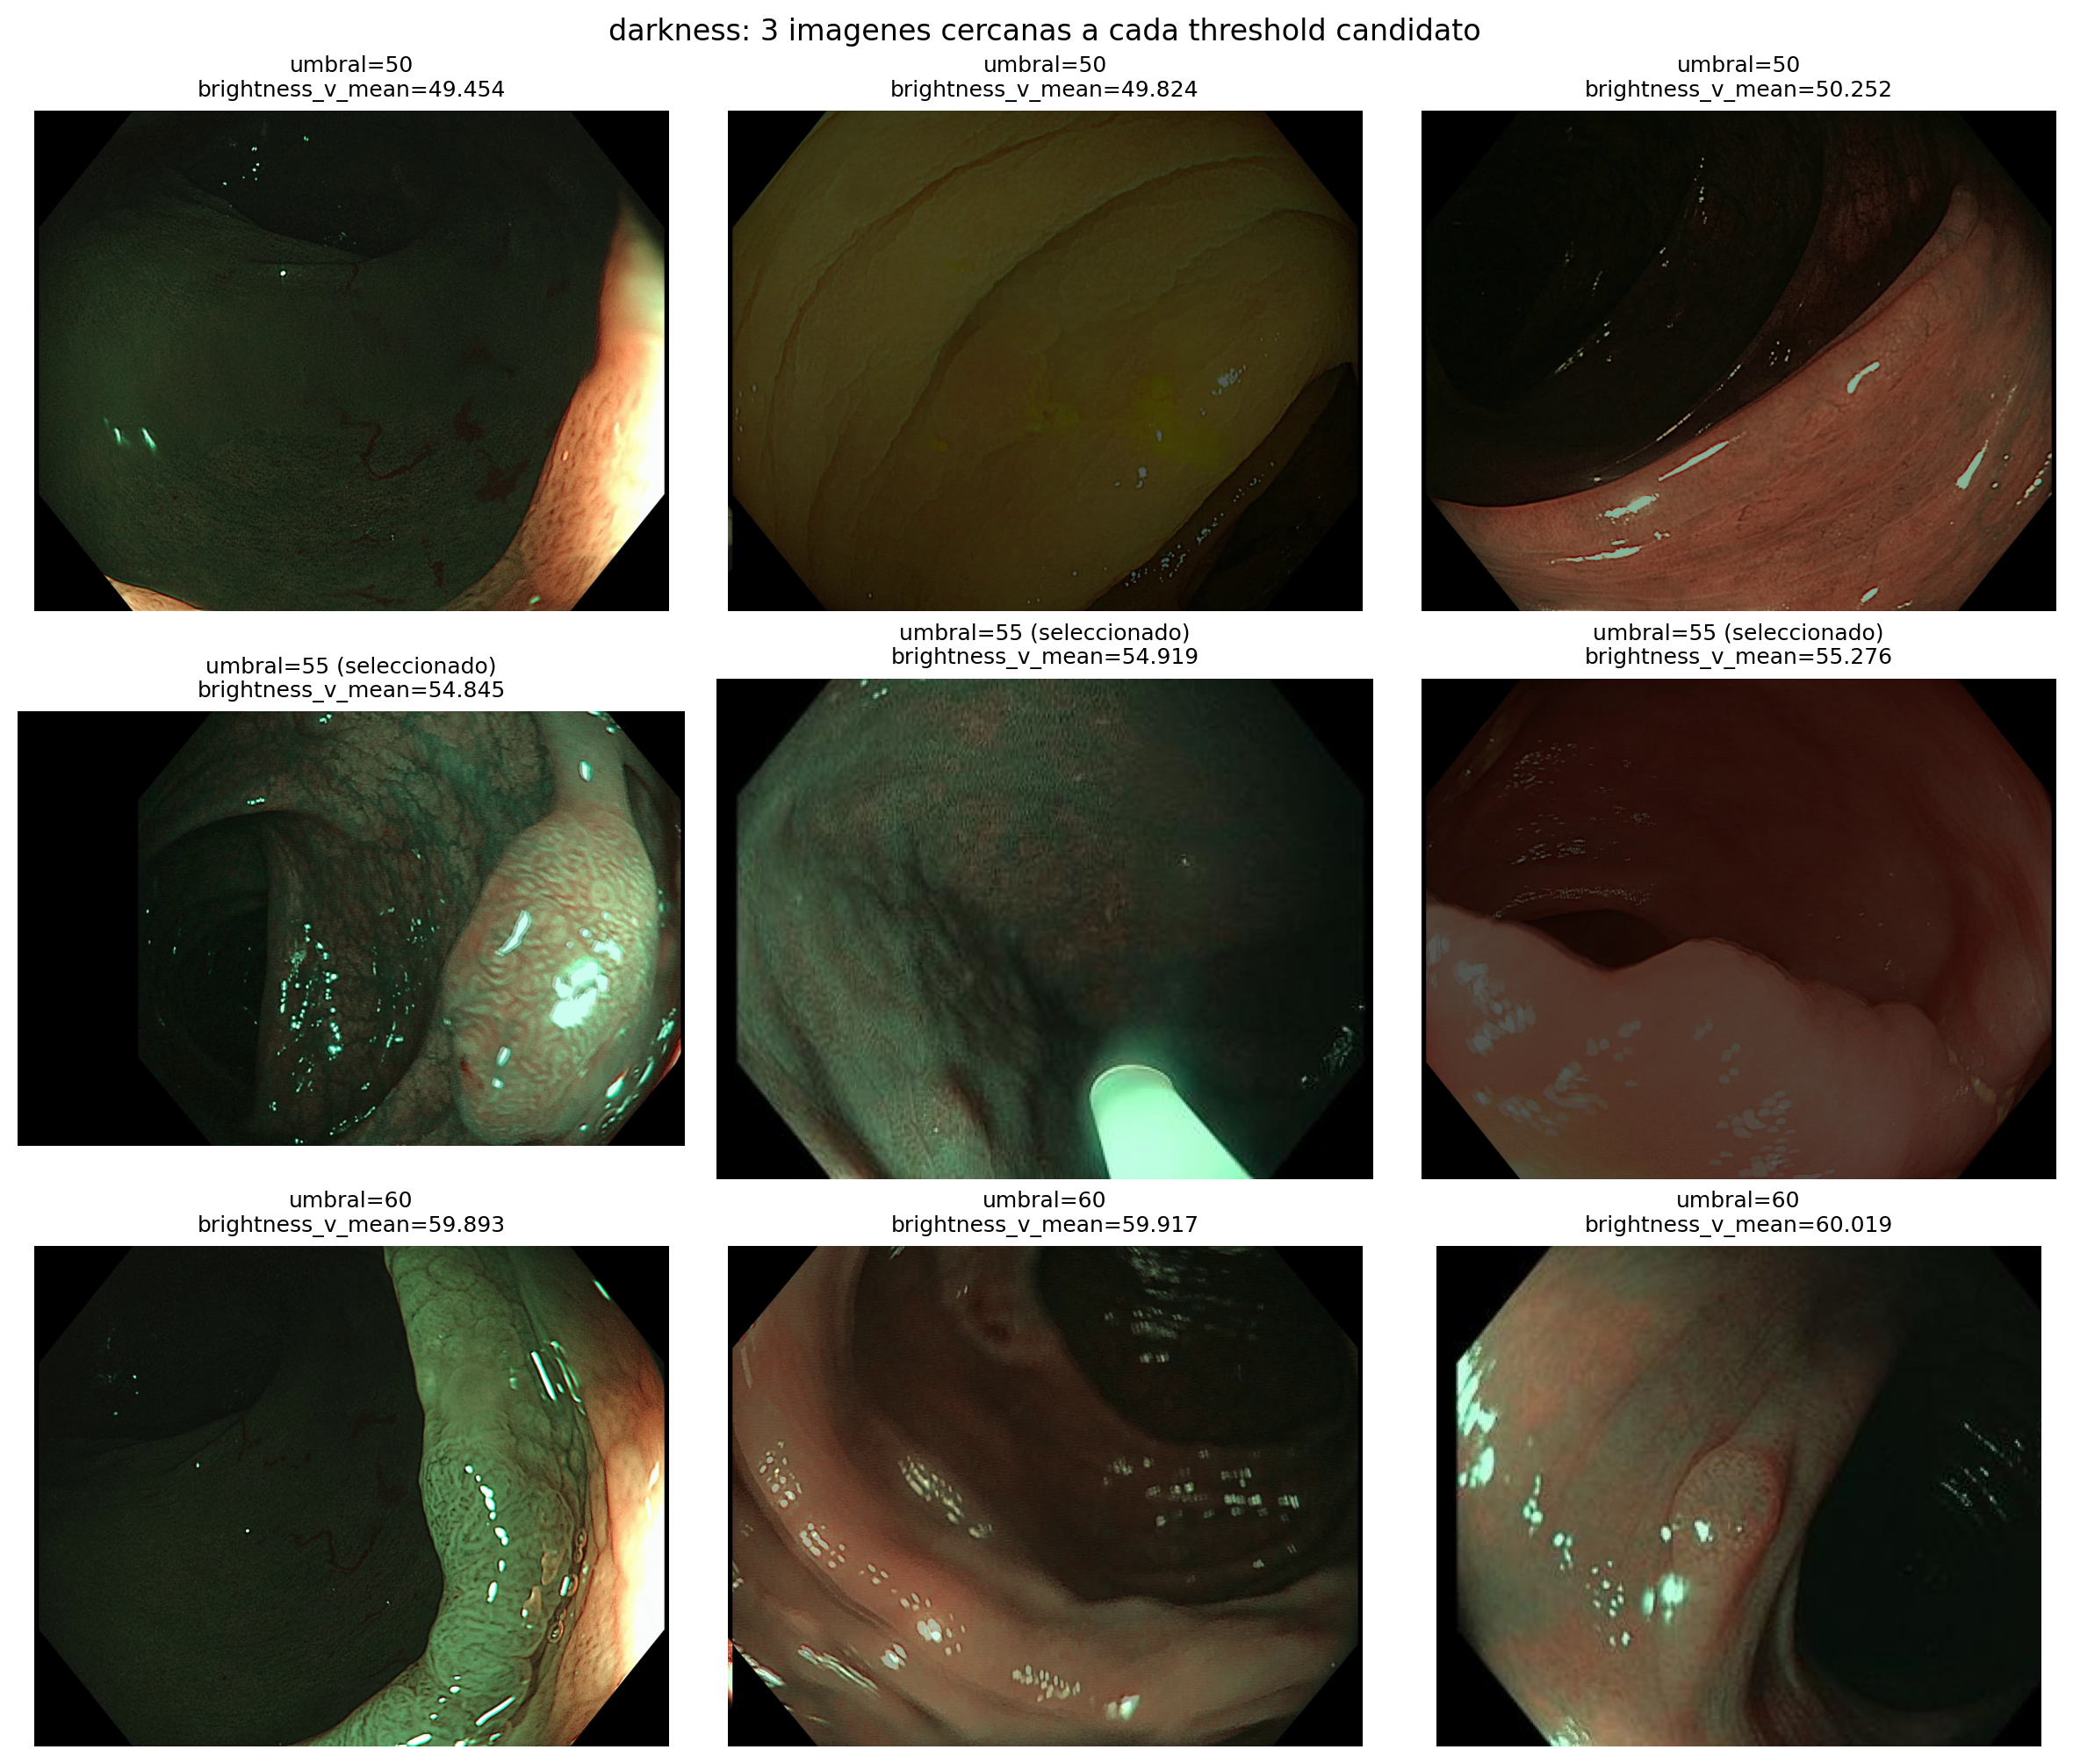
\includegraphics[width=\linewidth]{img/phase4_darkness_threshold_examples.png}
\captionof{figure}{Ejemplos cercanos a los umbrales candidatos del filtro de oscuridad.}
\label{fig:phase4_darkness_threshold}
\end{minipage}
\end{center}

\textbf{Filtro de uniformidad.} Elimina imágenes con muy poca estructura visual, típicamente producidas por contacto de la cámara con la mucosa. Para ello se calcula la entropía de Shannon en escala de grises. Si la entropía es inferior a $T_{uniform}=6.25$, el frame se descarta. Los valores candidatos evaluados son 6.0, 6.25 y 6.5, resumidos visualmente en la Figura~\ref{fig:phase4_uniformity_threshold}.

\begin{center}
\begin{minipage}{\linewidth}
\centering
\includegraphics[width=\linewidth]{img/phase4_uniformity_threshold_examples.png}
\captionof{figure}{Ejemplos cercanos a los umbrales candidatos del filtro de uniformidad.}
\label{fig:phase4_uniformity_threshold}
\end{minipage}
\end{center}

\textbf{Filtro de desenfoque.} Detecta imágenes borrosas mediante la varianza del Laplaciano. Si la varianza es inferior a $T_{lap}=25$, la imagen se considera insuficientemente nítida y se elimina. En este caso se comparan los valores candidatos 20, 25 y 30, tal como se muestra en la Figura~\ref{fig:phase4_blur_threshold}.

\begin{center}
\begin{minipage}{\linewidth}
\centering
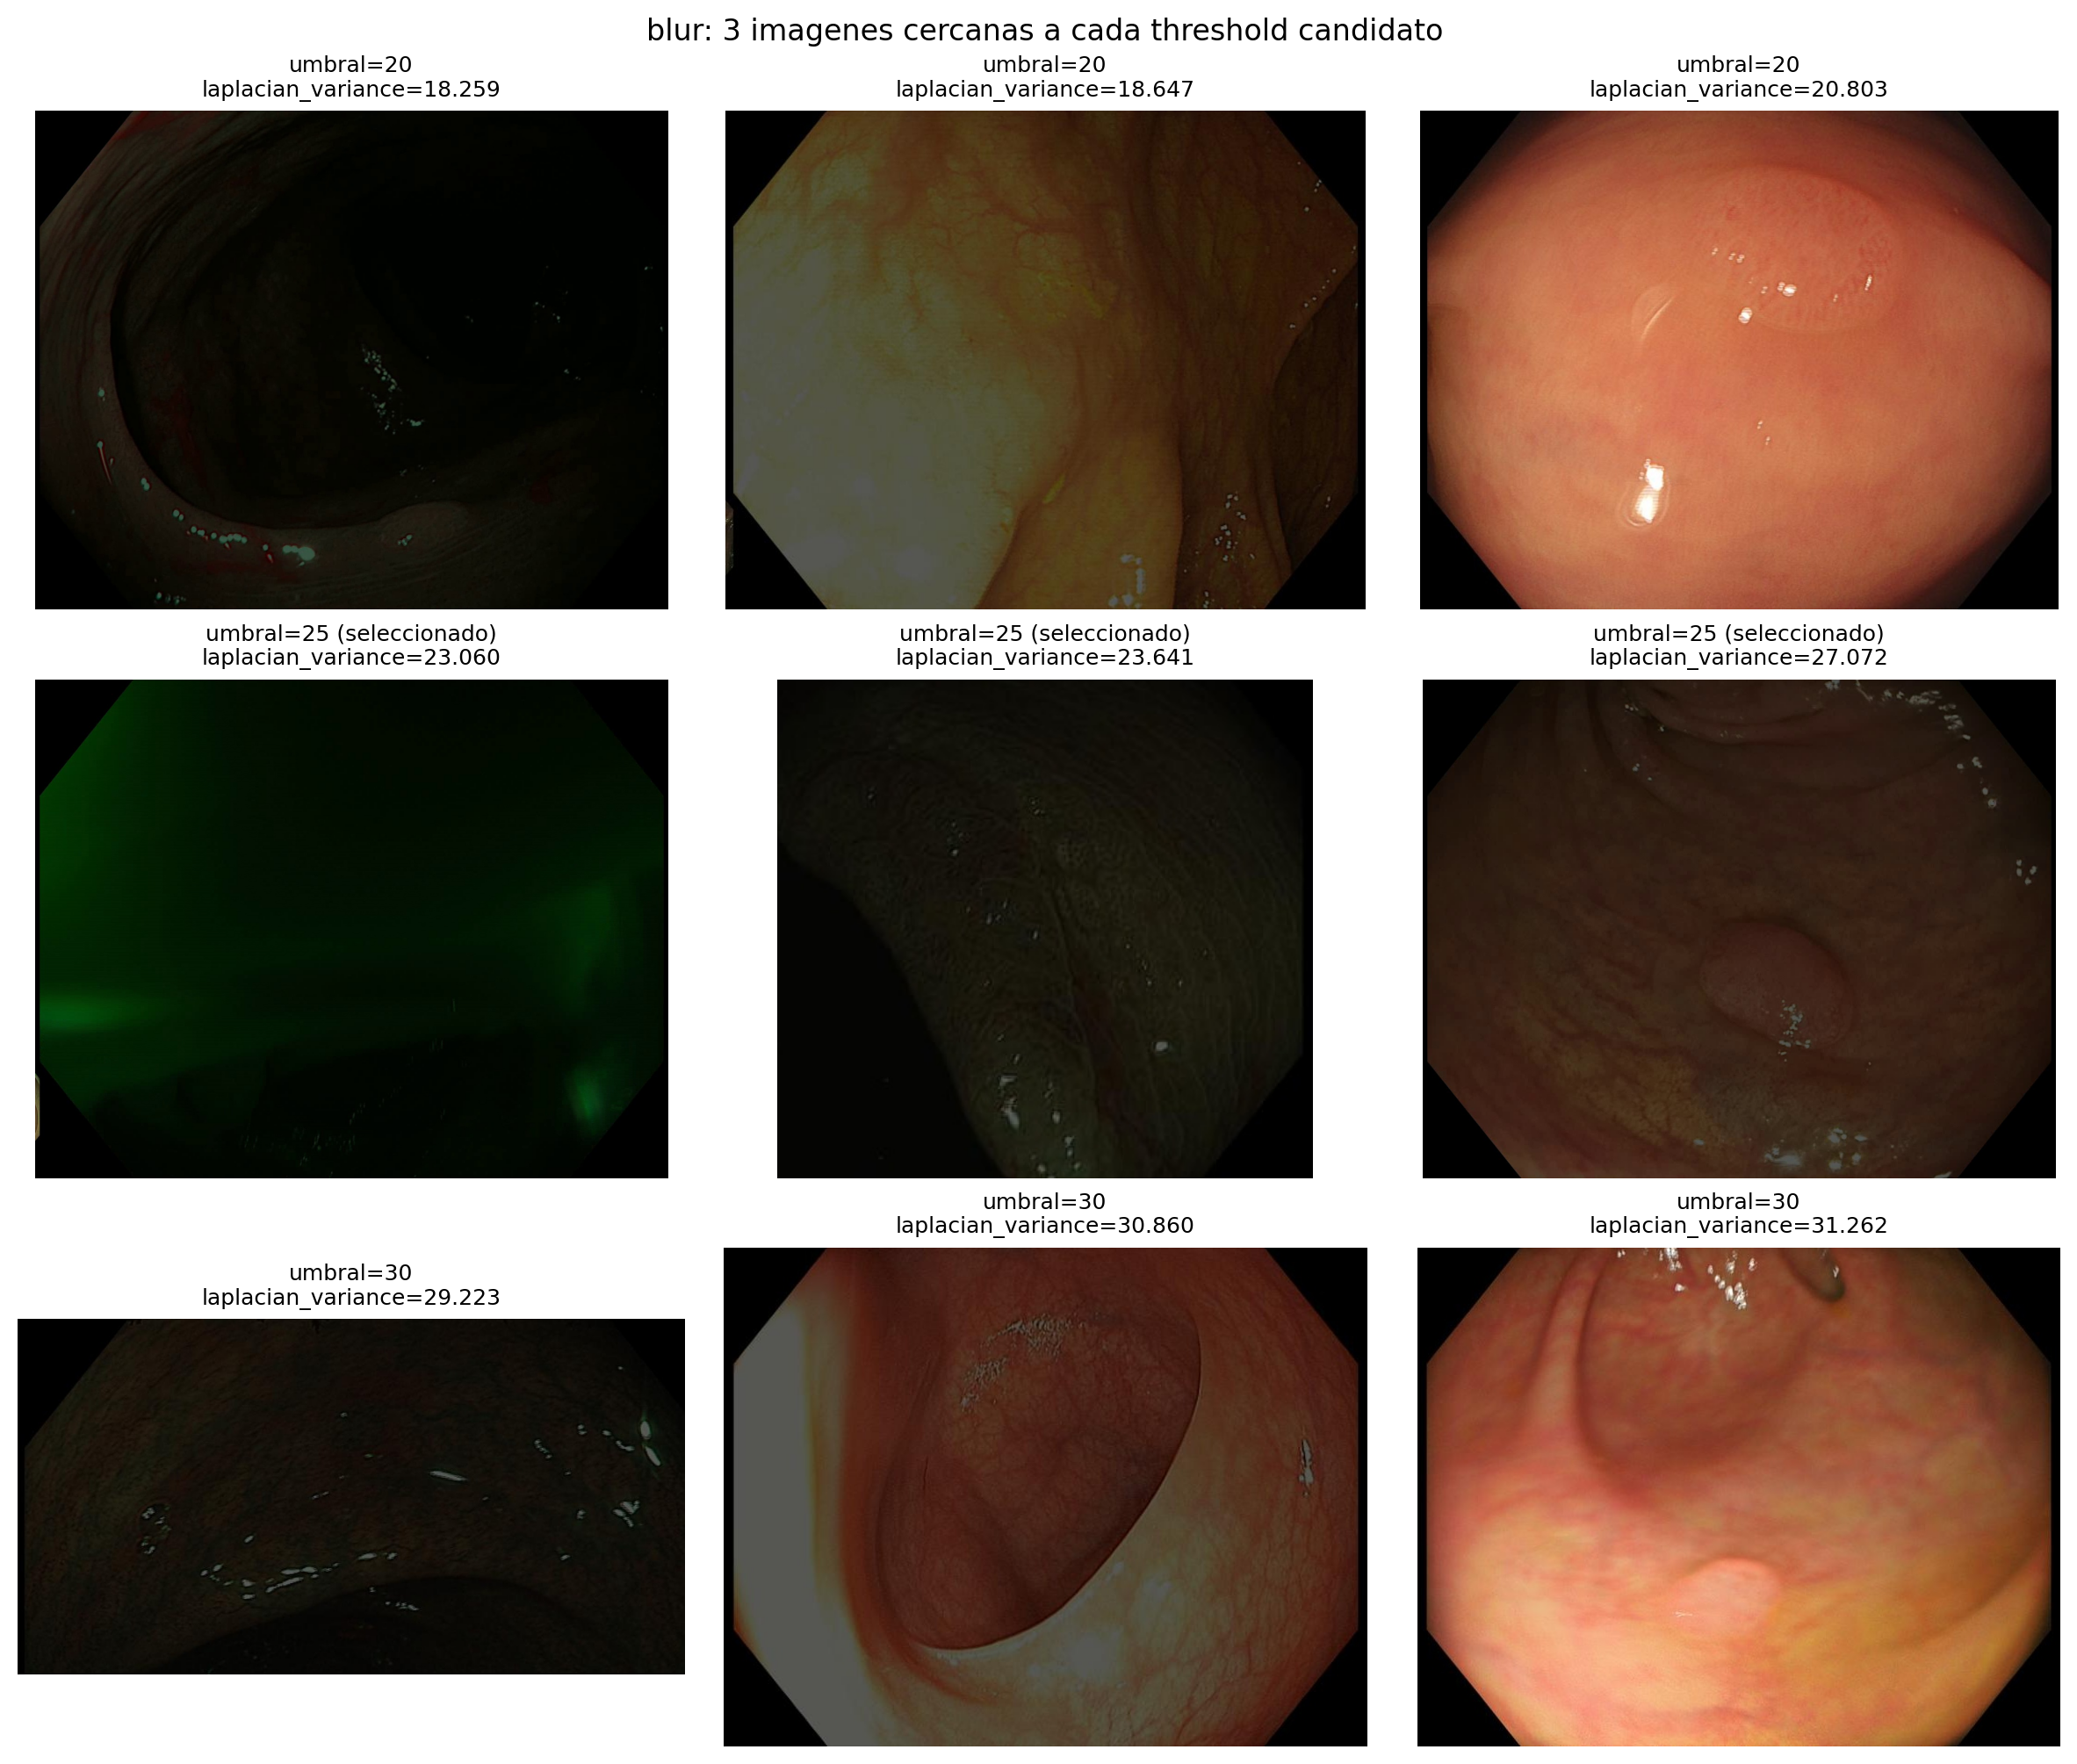
\includegraphics[width=\linewidth]{img/phase4_blur_threshold_examples.png}
\captionof{figure}{Ejemplos cercanos a los umbrales candidatos del filtro de desenfoque.}
\label{fig:phase4_blur_threshold}
\end{minipage}
\end{center}

El resultado de esta fase es un nuevo CSV de entrenamiento que conserva la misma estructura de metadata del pipeline, pero excluye las imágenes que no superan los criterios de calidad definidos. La validación no se modifica, manteniendo el protocolo experimental común del proyecto.

\section{Resultados y análisis}

\subsection{Protocolo experimental común}
Para evaluar el efecto de las fases del pipeline, el modelo \textit{baseline} se mantiene fijo y se modifica únicamente el conjunto de entrenamiento. La validación se realiza siempre sobre el mismo conjunto, definido en la fase 1, para que las comparaciones entre fases no dependan de cambios en la partición de evaluación.

La métrica principal es el F1-score macro, ya que otorga el mismo peso a todas las clases y resulta más informativa que la accuracy en un problema multiclase desbalanceado. De forma complementaria se reportan accuracy, balanced accuracy, weighted F1 y métricas por clase.

Es importante destacar que el baseline inicial se ha ejecutado con varias semillas para estimar la estabilidad del entrenamiento, mientras que los resultados de las fases posteriores corresponden por el momento a ejecuciones preliminares. En la versión final del trabajo se preve repetir los experimentos principales con el mismo protocolo de semillas, de modo que la comparacion entre fases no dependa de una unica ejecucion.

\subsection{Resultados de la fase 1: baseline}
El conjunto efectivo utilizado en la fase 1 contiene 3252 imágenes con etiqueta histológica válida. La Tabla~\ref{tab:phase1_split} muestra la distribución obtenida tras la partición estratificada y agrupada.

\begin{table}[t]
\centering
\small
\setlength{\tabcolsep}{4pt}
\caption{Distribución de clases en la fase 1}
\label{tab:phase1_split}
\resizebox{\columnwidth}{!}{%
\begin{tabular}{l r r r}
\hline
\textbf{Clase} & \textbf{Train} & \textbf{Validación} & \textbf{Total} \\
\hline
Adenoma & 1515 & 379 & 1894 \\
Sessile serrated adenoma & 671 & 168 & 839 \\
Hyperplastic & 319 & 80 & 399 \\
Adenocarcinoma & 100 & 20 & 120 \\
\hline
Total & 2605 & 647 & 3252 \\
\hline
\end{tabular}%
}
\end{table}

Para estimar la estabilidad del entrenamiento, el baseline se ejecuta con cuatro semillas distintas manteniendo fija la partición de validación. Los resultados globales se resumen en la Tabla~\ref{tab:phase1_results}.

\begin{table}[t]
\centering
\small
\setlength{\tabcolsep}{4pt}
\caption{Resultados del baseline en validación}
\label{tab:phase1_results}
\resizebox{\columnwidth}{!}{%
\begin{tabular}{r r r r r}
\hline
\textbf{Seed} & \textbf{Accuracy} & \textbf{Balanced Acc.} & \textbf{Macro F1} & \textbf{Weighted F1} \\
\hline
42 & 0.5255 & 0.5844 & 0.4864 & 0.5398 \\
123 & 0.4467 & 0.6062 & 0.4627 & 0.4505 \\
456 & 0.4915 & 0.6048 & 0.4738 & 0.5007 \\
789 & 0.4575 & 0.6035 & 0.4534 & 0.4596 \\
\hline
Media $\pm$ std & $0.4803 \pm 0.0357$ & $0.5997 \pm 0.0103$ & $0.4691 \pm 0.0143$ & $0.4876 \pm 0.0411$ \\
\hline
\end{tabular}%
}
\end{table}

El baseline alcanza un F1-score macro medio de 0.4691. Este resultado confirma la dificultad del problema y establece el punto de referencia sobre el que deben interpretarse las fases posteriores. La clase con peor comportamiento es \textit{Hyperplastic}, con un F1 medio de 0.2917, mientras que \textit{Adenocarcinoma} obtiene un recall elevado pero sobre un soporte de validación reducido. Este comportamiento refuerza la necesidad de actuar sobre la distribución y calidad del dataset, que es precisamente el objetivo principal del pipeline.

\subsection{Resultados de la fase 2: ingestión}
La ingestión desde vídeo genera un conjunto efectivo de entrenamiento de 7615 imágenes. De ellas, 2552 corresponden a imágenes originales normalizadas dentro del pipeline y 5063 son nuevos frames extraídos desde vídeo. El incremento no es uniforme entre clases, sino que se aplica de forma más intensa sobre las histologías menos representadas para reducir parcialmente el desbalanceo desde la propia generación de datos.

\begin{table}[t]
\centering
\small
\setlength{\tabcolsep}{4pt}
\caption{Composición del dataset tras la ingestión de vídeo}
\label{tab:phase2_distribution}
\resizebox{\columnwidth}{!}{%
\begin{tabular}{l r r r}
\hline
\textbf{Clase} & \textbf{Originales} & \textbf{Vídeo} & \textbf{Total} \\
\hline
Adenoma & 1466 & 1326 & 2792 \\
Sessile serrated adenoma & 667 & 1773 & 2440 \\
Hyperplastic & 319 & 1349 & 1668 \\
Adenocarcinoma & 100 & 615 & 715 \\
\hline
Total & 2552 & 5063 & 7615 \\
\hline
\end{tabular}%
}
\end{table}

Con el mismo protocolo de validación, el entrenamiento sobre el dataset ampliado obtiene un F1-score macro de 0.5617, frente al 0.4691 medio del baseline inicial. Las métricas globales de esta ejecución son: accuracy 0.5750, balanced accuracy 0.5779 y weighted F1 0.5798. La mejora absoluta de Macro F1 respecto a la media del baseline es de 0.0926. Este resultado sugiere que la incorporación controlada de frames procedentes de vídeo aporta variabilidad útil al entrenamiento. Al mismo tiempo, el fuerte aumento de muestras generadas justifica la necesidad de la fase posterior de deduplicación, ya que una parte de las imágenes añadidas puede ser temporalmente redundante.

\subsection{Resultados de la fase 3: deduplicación}
La deduplicación se aplica sobre las 7615 imágenes generadas tras la fase de ingestión. El proceso identifica 2092 grupos temporales y calcula 17327 comparaciones por pares. La Tabla~\ref{tab:phase3_pair_methods} muestra la distribución de los pares según los criterios de similitud cumplidos.

\begin{table}[t]
\centering
\small
\setlength{\tabcolsep}{4pt}
\caption{Clasificación de pares comparados en la deduplicación}
\label{tab:phase3_pair_methods}
\resizebox{\columnwidth}{!}{%
\begin{tabular}{l r}
\hline
\textbf{Criterio cumplido} & \textbf{Pares} \\
\hline
Ninguno & 11916 \\
Solo pHash & 3675 \\
Solo SSIM & 242 \\
SSIM y pHash & 1494 \\
\hline
Total & 17327 \\
\hline
\end{tabular}%
}
\end{table}

Como la versión actual solo considera redundantes los pares que cumplen ambos umbrales, se detectan 1494 pares redundantes. Estos pares conectan 846 imágenes dentro de componentes redundantes. Tras agrupar las redundancias y seleccionar los mejores frames de cada grupo, se conservan 7201 imágenes y se eliminan 414. Los valores \textit{top-K} utilizados en esta ejecución son 1 para adenomas, 2 para adenomas sésiles serrados, 2 para hiperplásicos y 4 para adenocarcinomas.

La distribución final tras esta fase queda menos redundante, pero sigue conservando una presencia elevada de las clases minoritarias: 2660 adenomas, 2330 adenomas sésiles serrados, 1510 hiperplásicos y 701 adenocarcinomas. El entrenamiento sobre el dataset deduplicado obtiene un F1-score macro de 0.5349 en validación, con accuracy 0.5502, balanced accuracy 0.5764 y weighted F1 0.5596.

Aunque la deduplicación reduce el F1-score macro respecto a la fase 2, su función principal no es aumentar el volumen de datos, sino controlar la redundancia temporal introducida por la ingestión desde vídeo. Al exigir que se cumplan simultáneamente los umbrales de SSIM y pHash, la fase se mantiene conservadora y evita eliminar variantes visuales que podrían seguir aportando información útil.

\subsection{Conclusiones provisionales}

Los resultados obtenidos hasta esta entrega apoyan parcialmente la hipotesis principal del trabajo: modificar sistematicamente el conjunto de entrenamiento puede mejorar el rendimiento de un modelo baseline fijo sin recurrir a arquitecturas más complejas. La fase de ingestión desde video produce la mejora más clara hasta el momento, aumentando el F1-score macro respecto al baseline inicial. Esto sugiere que los frames extraidos alrededor de las anotaciones clinicas aportan variabilidad visual util para el entrenamiento.

La fase de deduplicación reduce parte de la redundancia temporal introducida durante la ingestion. Aunque el F1-score macro disminuye respecto a la fase anterior, el resultado sigue siendo superior al baseline inicial. Esta fase debe interpretarse como un mecanismo de control de redundancia y no unicamente como una tecnica orientada a maximizar la metrica de forma inmediata.

La fase de filtrado de calidad queda como el principal bloque pendiente. Su ejecución permitirá comprobar si la eliminacion de imagenes con baja iluminacion, baja textura o desenfoque mejora la robustez del conjunto curado. Como trabajo inmediato, tambien queda pendiente revisar la estabilidad de los resultados mediante nuevas ejecuciones y analizar si la receta de entrenamiento actual requiere pequeños ajustes sin alterar el enfoque Data-Centric del proyecto.

\section{Uso de IA}
Durante el desarrollo de este proyecto se han utilizado como apoyo en dos tipos de tareas. En primer lugar, se ha utilizado para la revisión formal del texto, incluyendo aspectos de corrección lingüística y reformulación de párrafos ya redactados. En segundo lugar, se han utilizado como apoyo para comprender conceptos técnicos de visión por computador y deep learning no estudiados previamente.

La herramienta empleada con este fin ha sido Gemini, específicamente el modelo 3.1\cite{google_gemini_2026}

\bibliographystyle{ieeetr}
\bibliography{referencias}

\end{document}
